\section{Design of Tectonic}

\subsection{Tectonic Architecture}\label{sec:tectonic_architecture}

A Tectonic cluster is composed of Chunk Stores, Metadata Stores, and Background Services. A Client Library, tailored for various Tectonic use cases, interfaces with the Metadata and Chunk Stores to store and retrieve data. The architecture of Tectonic is illustrated in \Cref{fig:tectonic_architecture}, with additional details provided in the subsequent sections. Tectonic clusters are resilient to host, rack, and power failures at the data center level. For geo-replication, tenants can deploy multiple Tectonic clusters across different data centers.

\begin{figure}[htbp]
    \centering
    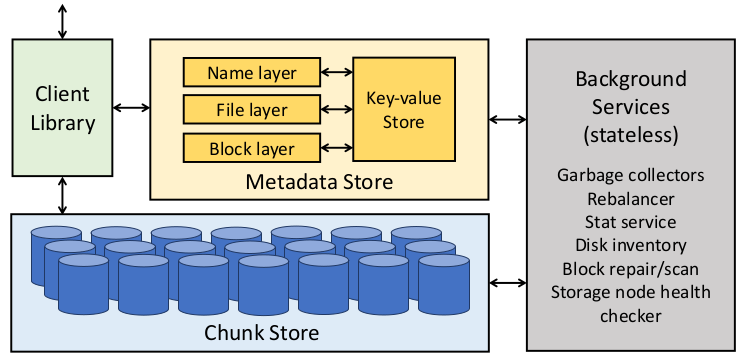
\includegraphics[width=0.8\textwidth]{pics/design.png}
    \caption{Tectonic architecture, with arrows indicating network calls. Filesystem metadata is stored in a key-value store. All components are stateless, except for the Chunk and Metadata Stores.}\label{fig:tectonic_architecture}
\end{figure}

\subsubsection{Chunk Store}\label{sec:chunk_store}
In Tectonic, a file is composed of multiple blocks, each containing several chunks, which are the fundamental data storage unit. The Chunk Store is a flat, distributed object store that manages these chunks and is designed to scale linearly with the number of storage nodes, supporting exabytes of data. This abstraction is managed by the Client Library and the Metadata Store, which handle higher-level abstractions like blocks and files.

Chunks are stored as files on storage nodes, each running a local instance of XFS. These nodes are equipped with 36 hard drives for chunk storage and a 1 TB SSD for XFS metadata and caching frequently accessed chunks. The SSD cache is managed using a flash endurance-aware caching library to optimize performance. Tectonic ensures block durability through Reed-Solomon (RS) encoding or replication. Chunks within blocks are distributed across fault domains for fault tolerance, and background services repair damaged or lost chunks to maintain data durability.

\subsubsection{Metadata Store}\label{sec:metadata_store}
Tectonic addresses the challenge of managing large volumes of metadata by organizing it hierarchically into multiple layers. The Metadata Store is a distributed key-value store, divided into three distinct layers:

\begin{itemize}\label{list:metadata_layers}
    \item \textbf{Name Layer}: Maps directories to the sub-directories and files they contain.
    \item \textbf{File Layer}: Maps files to their associated blocks.
    \item \textbf{Block Layer}: Maps blocks to their corresponding chunks and includes a reverse mapping from chunks to blocks, which aids in garbage collection.
\end{itemize}

Unlike traditional directory mappings where a key maps to a list of values, Tectonic stores keys in an expanded format to enable faster updates. For example, if directory \texttt{A} contains sub-directory \texttt{B} and file \texttt{C}, the keys stored will be \texttt{(A, B)} and \texttt{(A, C)}, rather than a single key \texttt{A} mapping to both \texttt{B} and \texttt{C}. This approach accelerates updates and eliminates the need for locks during the update process. However, listing the contents of a directory requires a prefix scan over the keys.

Another design choice is the use of hash partitioning for the different layers, instead of range partitioning. This method provides better load balancing and helps prevent hotspots in the system, particularly for Data Warehouse parallel processing workloads, as discussed in \Cref{sec:data_warehouse}.

At a lower level, the Metadata Store is powered by ZippyDB \cite{zippydb}, with each node using RocksDB \cite{rocksdb} for storing key-value pairs. Fault tolerance is ensured through replication, utilizing the Paxos consensus protocol \cite{paxos}.

While this design enables scalability and mitigates hotspots, it introduces some challenges. The layered architecture results in increased latency for metadata operations. To address this, Tectonic clients can seal directories, which allows for caching of metadata within the client library. Furthermore, Tectonic does not support atomic cross-directory operations, nor does it provide a direct API for listing the entire contents of a directory. Consequently, clients are required to implement a wrapper around the list API to retrieve the contents of a directory.


\subsubsection{Client Library} \label{sec:client_library}

The Client Library provides a filesystem abstraction using the metadata, operating at the chunk granularity for read and write operations. It enforces \textbf{Single Writer Semantics} by issuing a token when a client opens a file for appending. This token must accompany all subsequent metadata updates, ensuring that only the last process to open the file can perform writes.

For multiple-writer semantics, tenants can implement custom serialization protocols on top of Tectonic. Since the filesystem is intended for internal clients, such protocols are manageable and can be handled by the organization's developers using Tectonic for their specific use cases.


\subsubsection{Background Services} \label{sec:background_services}

Background services ensure consistency, durability, and efficient data management in Tectonic. These services maintain metadata consistency between layers, repair lost data, rebalance storage across nodes, and handle rack drains. They also publish statistics on filesystem usage.

The background services operate on one shard at a time, similar to the Metadata Store. Key services include a garbage collector that cleans up metadata inconsistencies (e.g., caused by failed Client Library operations or lazy object deletion), and a rebalancer and repair service that work together to relocate or delete chunks. The rebalancer identifies chunks needing relocation due to events like hardware failures or increased storage capacity, while the repair service handles the actual data movement, operating on a per-Block layer shard and per-disk basis to scale horizontally. The block layer and the rebalancer service work together to ensure that the total number of copysets\cite{copyset} is maintained, and that chunks are distributed evenly across nodes. 

A copyset refers to a group of replicas of a data chunk stored across different nodes. The system ensures that each chunk of data has multiple copies distributed across multiple nodes to protect against node failures. The copyset concept ensures that even in the event of hardware or network failures, data availability and durability are maintained by limiting the total number of distinct copysets in the system. Each chunk belongs to a specific copyset, and the number of replicas (copysets) is dynamically managed based on system requirements such as redundancy levels, storage capacity, and load balancing.


\subsection{Multitenancy}\label{sec:multitenancy}

Tectonic categorizes resources into two types: \textbf{non-ephemeral} and \textbf{ephemeral}. Non-ephemeral resources change slowly over time and typically do not have dynamic adjustment semantics. An example of this is the storage capacity allocated to a tenant, which is pre-configured and remains static.

In contrast, ephemeral resources change rapidly and require dynamic monitoring and automated adjustments. Examples include storage IOPS capacity and metadata query capacity.

One key challenge is determining the appropriate level at which to manage resources. Providing isolation at the application level is complex due to the difficulty of managing resources across multiple applications. On the other hand, isolation at the tenant level may be too generalized. To address this, Tectonic introduces the concept of \texttt{TrafficGroup} and \texttt{TrafficClass} for managing resources. A \texttt{TrafficGroup} consists of applications with similar storage requirements within a tenant, and each \texttt{TrafficGroup} is assigned a \texttt{TrafficClass}. Tectonic defines three types of \texttt{TrafficClass}: \texttt{Gold} (Latency-sensitive), \texttt{Silver} (Normal), and \texttt{Bronze} (Background services). Tectonic manages resource access both at the global level and per node.

\subsubsection{Global Resource Management}\label{sec:global_resource_management}

The goal of global resource management is twofold: to limit resource usage and to efficiently share surplus resources across tenants. To achieve this, Tectonic employs a modified version of the leaky bucket algorithm, utilizing high-performance, near-real-time distributed counters.

The resource management process works as follows:

\begin{itemize}\label{list:resource_management}
    \item A resource counter is incremented for the corresponding \texttt{TrafficGroup} whenever a resource is used.
    \item If spare capacity is available, it is allocated for use.
    \item If a tenant exceeds its allocated capacity, the system checks for surplus capacity within other \texttt{TrafficGroups} of the same tenant.
    \item If no surplus capacity is found, the system then checks for spare capacity in other tenants.
\end{itemize}

When sharing resources between \texttt{TrafficGroups}, the request is treated as the \texttt{TrafficClass} of the lower-priority group. For example, if a \texttt{Gold} \texttt{TrafficGroup} requests resources from a \texttt{Silver} \texttt{TrafficGroup}, the request is treated as \texttt{Silver}. This prevents excessive increases in high-priority traffic, ensuring that the system remains stable and that many \texttt{Gold} requests can still meet their requirements.

\subsubsection{Per-Node Resource Management}\label{sec:per_node_resource_management}

The aim of per-node resource management is to prevent hotspots and ensure that the latency requirements for high-priority traffic, such as \texttt{Gold} class traffic, are met.

To achieve this, a Weighted Round-Robin (WRR) scheduling approach is employed. In this scheme, a request is skipped if its quota has already been used or if granting it would exceed the quota.

Several optimizations are applied to improve resource utilization:

\begin{itemize}
    \item Lower-priority request classes can yield their turn to higher-priority requests if there will still be enough time to service the lower-priority requests afterward.
    \item The number of non-\texttt{Gold} traffic requests in the queue for a disk is limited if there are pending \texttt{Gold} requests.
    \item Disks may rearrange requests to prioritize higher-priority traffic. If a \texttt{Gold} request is pending for a certain threshold amount of time, non-\texttt{Gold} requests may be deferred to prioritize the \texttt{Gold} request.
\end{itemize}

It is important to note that resource sharing at the node level is unnecessary, as it has already been handled globally.

\subsubsection{Access Control}\label{sec:access_control}

Tectonic employs a token-based access control mechanism to ensure that only authorized clients can access the system. In this system, each layer generates a token that must be included in subsequent requests to the next layer. The token is piggybacked on the request-reply. This mechanism effectively controls access by verifying the presence of a valid token in each request.

\subsection{Tenant-Specific Optimizations}\label{sec:tenant_specific_optimizations}

As mentioned in \Cref{sec:client_library}, the client library communicates directly with the chunk stores at the chunk granularity. This approach enables the optimization of read and write operations for specific tenants.

\subsubsection{Data Warehouse Write Optimizations}\label{sec:data_warehouse_optimization}

Data Warehouse storage has read after complete write semantics that is data is only read after the write operation is complete. This allows for optimizations such as: 

\subsubsection*{Asynchronous Writes}\label{sec:asynchronous_writes}

To optimize write operations, applications buffer writes until enough data is accumulated to form a block of the desired size. RS-Encoding is then done at the client itself, reducing the amount of data that needs to be transmitted to different nodes. This approach also reduces the number of network calls and disk seeks, enhancing write performance.

Importantly, there is no inconsistency introduced because metadata is only updated after the complete write operation has been successfully finished. This approach guarantees that data consistency is maintained throughout the write process.

\subsubsection*{Hedged Quorum Writes}

Hedged quorum writes aim to improve write latency by sending reservation requests to more nodes than the minimum required for a successful operation. Rather than waiting for the write to complete on all nodes, the system only waits until a majority of blocks have been successfully written, at which point the client is notified. 

This method effectively reduces the 99th percentile latency, enhancing the system's responsiveness and providing faster acknowledgment to clients.

\subsubsection{Blob Storage Optimizations}\label{sec:blob_storage_optimization}

\subsubsection*{Consistent Partial Block Appends}

To optimize append operations in blob storage, the system ensures that appends are consistent by waiting until the quorum size of appends is reached. This ensures data integrity and reduces unnecessary writes. Additionally, only the block creator is allowed to perform append operations, maintaining consistency and preventing data corruption.

Once an append operation is completed, the metadata is updated with the post-append block size and its corresponding checksum, ensuring consistency and reliability in the storage system.

\subsubsection*{Reencoding Blocks for Storage Efficiency}

Reencoding blocks for storage efficiency is made possible by the Client Library-driven design. Unlike traditional file systems, which typically require preconfiguration for file storage, this design allows more flexibility in optimizing storage. Specifically, blocks are reencoded from replicated formats to Reed-Solomon (RS) after a certain amount of time has passed. This process reduces the storage overhead associated with replication, enhancing storage efficiency and reducing costs.
